\documentclass{article}
\usepackage{tikz}
\usetikzlibrary{external}
\tikzexternalize[prefix=]

\usepackage{amsmath,amssymb,amsfonts,mathrsfs}
\usepackage{siunitx}
\usepackage{mathtools}

\usepackage[utf8]{inputenc}
\usepackage{pgfplots}
\DeclareUnicodeCharacter{2212}{−}
\usepgfplotslibrary{groupplots,dateplot}
\usetikzlibrary{patterns,shapes.arrows}
\pgfplotsset{compat=newest}
\usetikzlibrary{arrows}
\usepackage{xcolor}

\begin{document}
% This file was created with tikzplotlib v0.10.1.
% This file was created with tikzplotlib v0.10.1.
% This file was created with tikzplotlib v0.10.1.
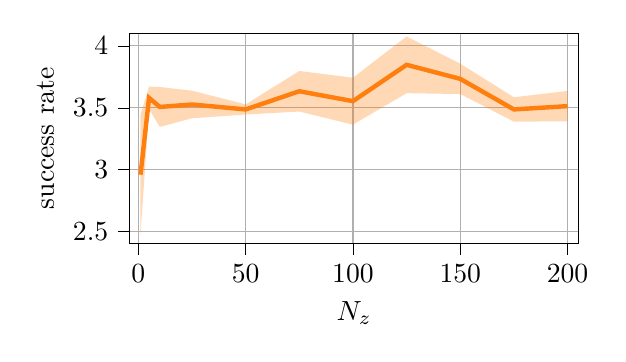
\begin{tikzpicture}

\definecolor{darkgray176}{RGB}{176,176,176}
\definecolor{steelblue31119180}{RGB}{31,119,180}
\definecolor{darkorange25512714}{RGB}{255,127,14}


\begin{axis}[
tick align=outside,
tick pos=left,
x grid style={darkgray176},
xlabel={\(\displaystyle N_z\)},
xmajorgrids,
xmin=-3.95, xmax=204.95,
xtick style={color=black},
y grid style={darkgray176},
ylabel={success rate},
ymajorgrids,
ymin=2.4086432397869, ymax=4.1,
ytick style={color=black},
legend style={at={(0.9,0.3)}},
    width=0.6\textwidth,
    height=0.35\textwidth,
]
% \begin{axis}[
% tick align=outside,
% tick pos=left,
% x grid style={darkgray176},
% xmin=-3.95, xmax=104.95,
% xtick style={color=black},
% y grid style={darkgray176},
% ymin=2.4086432397869, ymax=3.86301227189616,
% ytick style={color=black}
% ]
\path [fill=darkorange25512714, opacity=0.3]
(axis cs:1,3.44524907693541)
--(axis cs:1,2.47475092306459)
--(axis cs:5,3.48907878868676)
--(axis cs:10,3.34555938701874)
--(axis cs:25,3.41551111999645)
--(axis cs:50,3.44557057331354)
--(axis cs:75,3.4697620780482)
--(axis cs:100,3.36406573911229)
--(axis cs:125,3.61785330264359)
--(axis cs:150,3.61076815792766)
--(axis cs:175,3.38823451293178)
--(axis cs:200,3.39076815792766)
--(axis cs:200,3.635898508739)
--(axis cs:200,3.635898508739)
--(axis cs:175,3.58509882040156)
--(axis cs:150,3.855898508739)
--(axis cs:125,4.07548003068974)
--(axis cs:100,3.74260092755438)
--(axis cs:75,3.79690458861847)
--(axis cs:50,3.52776276001979)
--(axis cs:25,3.63782221333689)
--(axis cs:10,3.66777394631459)
--(axis cs:5,3.67092121131324)
--(axis cs:1,3.44524907693541)
--cycle;

\addplot [ultra thick, darkorange25512714]
table {%
1 2.96
5 3.58
10 3.50666666666667
25 3.52666666666667
50 3.48666666666667
75 3.63333333333333
100 3.55333333333333
125 3.84666666666667
150 3.73333333333333
175 3.48666666666667
200 3.51333333333333
};
\end{axis}

\end{tikzpicture}




\end{document}